\documentclass[14pt,tikz,border=12pt]{standalone}

% --- Better poster typography ---
\usepackage[T1]{fontenc}
\usepackage{tgheros}          % TeX Gyre Heros (Helvetica-like)
\usepackage[final]{microtype} % nicer spacing/kerning
\renewcommand{\familydefault}{\sfdefault}

\usepackage{xcolor}
\usepackage{tikz}
\usetikzlibrary{arrows.meta,positioning,shadows.blur,fit}

% --------- Theme Palette ---------
\definecolor{farsun}{HTML}{1F77B4}   % FARSuN blue
\definecolor{silso}{HTML}{FF7F0E}    % SILSO orange
\definecolor{rob}{HTML}{2CA02C}      % ROB green
\definecolor{plum}{HTML}{9467BD}     % accent purple
\definecolor{slate}{HTML}{1F2937}    % deep slate

\colorlet{axisline}{slate}
\colorlet{milestone}{slate}
\colorlet{card25}{farsun!88}
\colorlet{card26}{plum!82}
\colorlet{card26d}{plum!90!black}
\colorlet{card27}{silso!85}
\colorlet{card267}{rob!88!black}

% --- Title/body helpers (use these in card text) ---
\newcommand{\CardTitle}[1]{{\bfseries\LARGE #1}}
\newcommand{\CardText}[1]{{\bfseries\normalsize #1}}

\begin{document}
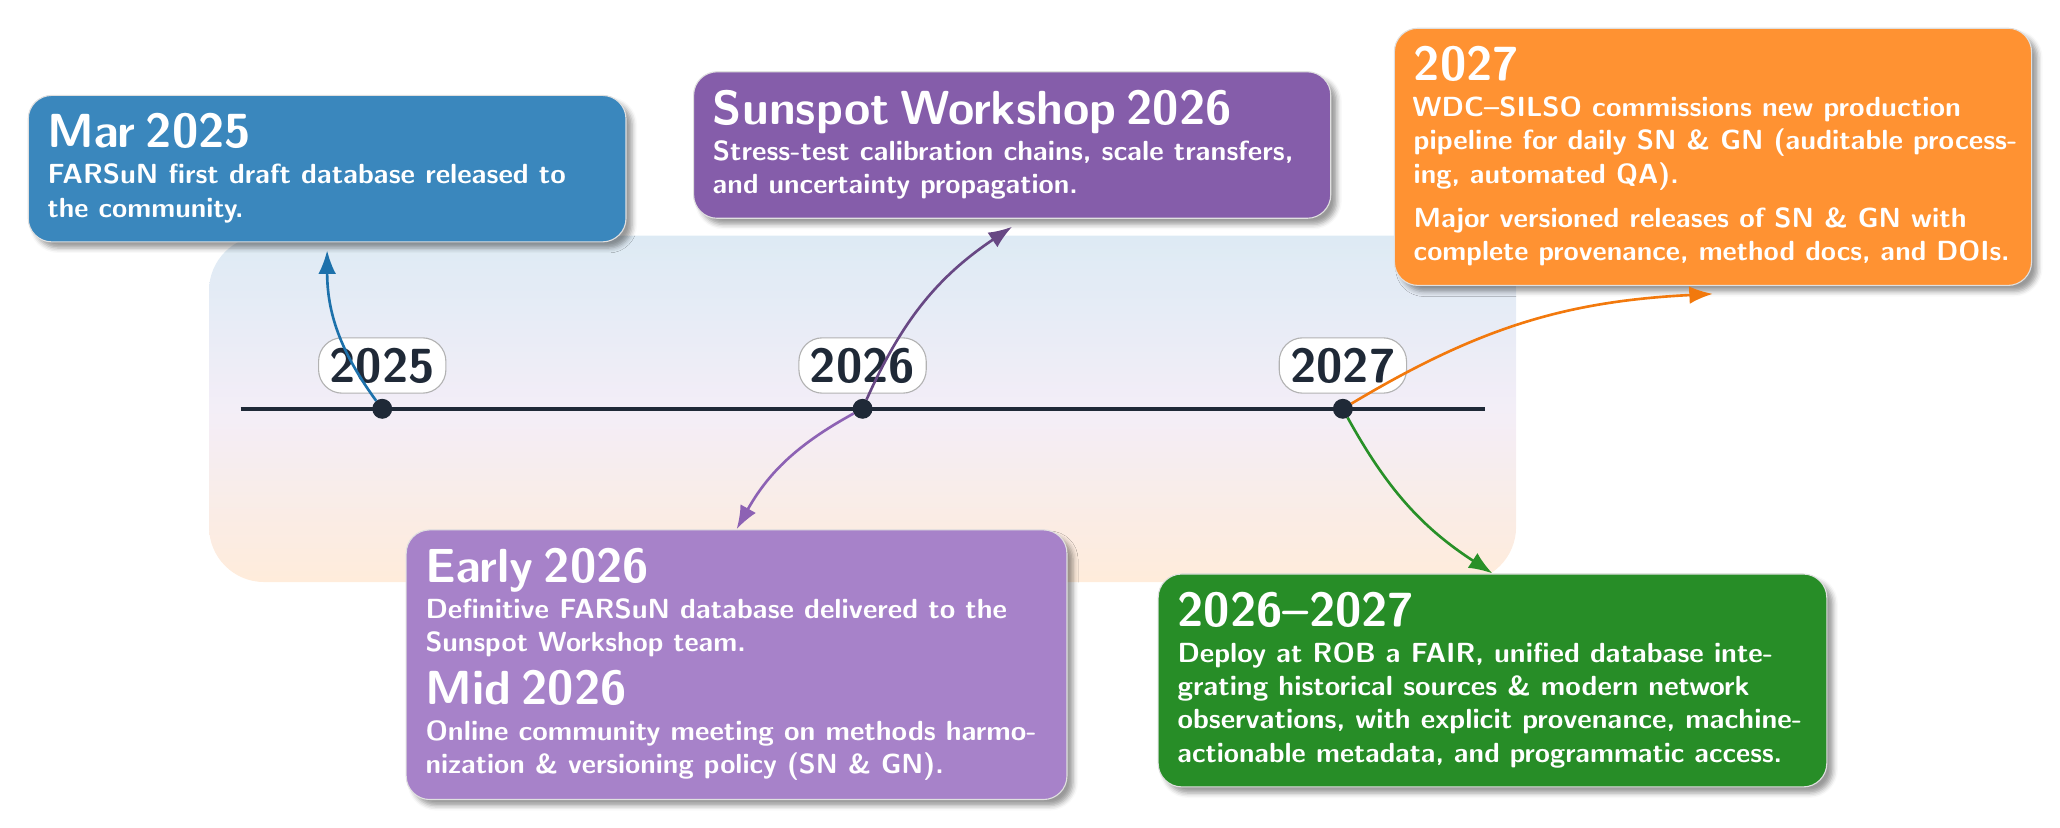
\begin{tikzpicture}[
  every node/.style={font=\bfseries},        % body text bold by default
  axis/.style={line width=1.25pt, draw=axisline},
  milestone/.style={circle, draw=milestone, fill=milestone, inner sep=2.4pt},
  card/.style={
    rectangle, rounded corners=3mm,
    align=left, draw=black!12, text=white,
    inner sep=7pt, blur shadow
  },
  leader/.style={-{Latex[length=3mm]}, line width=0.95pt},
  yearchip/.style={
    rounded corners=3mm, fill=white, draw=black!30,
    inner sep=4pt, font=\bfseries\LARGE, text=slate
  }
]

% ---------- Geometry ----------
\def\yearsep{6.1}
\coordinate (Y2025) at (0,0);
\coordinate (Y2026) at (\yearsep,0);
\coordinate (Y2027) at (2*\yearsep,0);

% ---------- Background gradient ribbon ----------
\begin{scope}
  \path[rounded corners=7mm, draw=none,
        left color=farsun!16, right color=silso!16, middle color=plum!12,
        shading=axis, shading angle=0, opacity=0.95]
        ($(Y2025)+(-2.2,2.2)$) rectangle ($(Y2027)+(2.2,-2.2)$);
\end{scope}

% ---------- Axis + milestones ----------
\draw[axis] ($(Y2025)+(-1.8,0)$) -- ($(Y2027)+(1.8,0)$);
\node[milestone] (M25) at (Y2025) {};
\node[milestone] (M26) at (Y2026) {};
\node[milestone] (M27) at (Y2027) {};

% ---------- Year chips ----------
\node[yearchip] at ($(Y2025)+(0,0.55)$) {2025};
\node[yearchip] at ($(Y2026)+(0,0.55)$) {2026};
\node[yearchip] at ($(Y2027)+(0,0.55)$) {2027};

% ---------- Cards (use \CardTitle and \CardText) ----------
\node[card, fill=card25, text width=7.1cm] (C25a)
  at ($(Y2025)+(-0.7, 3.05)$) {
  \CardTitle{Mar 2025}\\[1pt]
  \CardText{FARSuN \emph{first draft database} released to the community.}
};

\node[card, fill=card26, text width=7.9cm] (C26a)
  at ($(Y2026)+(-1.6,-3.25)$) {
  \CardTitle{Early 2026}\\[1pt]
  \CardText{Definitive FARSuN database delivered to the Sunspot Workshop team.}\\[4pt]
  \CardTitle{Mid 2026}\\[1pt]
  \CardText{Online community meeting on methods harmonization \& versioning policy (SN \& GN).}
};

\node[card, fill=card26d, text width=7.6cm] (C26b)
  at ($(Y2026)+( 1.9, 3.35)$) {
  \CardTitle{Sunspot Workshop 2026}\\[1pt]
  \CardText{Stress-test calibration chains, scale transfers, and uncertainty propagation.}
};

\node[card, fill=card267, text width=8.0cm] (C267)
  at ($(Y2027)+(1.9,-3.45)$) {
  \CardTitle{2026--2027}\\[1pt]
  \CardText{Deploy at ROB a FAIR, unified database integrating historical sources \& modern network observations, with explicit provenance, machine-actionable metadata, and programmatic access.}
};

\node[card, fill=card27, text width=7.6cm] (C27a)
  at ($(Y2027)+( 4.7, 3.20)$) {
  \CardTitle{2027}\\[1pt]
  \CardText{WDC--SILSO commissions new production pipeline for daily SN \& GN (auditable processing, automated QA).}\\[4pt]
  \CardText{Major versioned releases of SN \& GN with complete provenance, method docs, and DOIs.}
};

% ---------- Leaders ----------
\draw[leader, draw=farsun!95!black] (M25) to[bend left=18] ($(C25a.south)+(0,-0.1)$);
\draw[leader, draw=plum!95!black] (M26) to[bend right=16] ($(C26a.north)+(0,0.0)$);
\draw[leader, draw=plum!70!black] (M26) to[bend left=16]  ($(C26b.south)+(0,-0.1)$);
\draw[leader, draw=rob!90!black]  (M27) to[bend right=14] ($(C267.north)+(0,0.0)$);
\draw[leader, draw=silso!95!black](M27) to[bend left=14]  ($(C27a.south)+(0,-0.1)$);

\end{tikzpicture}
\end{document}
